% the following command is only required if the thesis is written in german
\RequirePackage[ngerman=ngerman-x-latest]{hyphsubst}

\documentclass[
  ngerman, % change to ngerman for german theses
  symmetric, % use two-side for booklike layouts
  numbers=noenddot % remove trailing dots in chapter/section/... enumeration
]{tudscrreprt}
% use a custom serif font
\usepackage[bitstream-charter]{mathdesign}
% make chapter, section, ... use serif font
\addtokomafont{disposition}{\rmfamily}

\usepackage[T1]{fontenc}
\usepackage[utf8]{inputenc}
\usepackage[
  ngerman % change to ngerman for german theses
]{babel}
\usepackage{isodate}
\usepackage{pdfpages}
\usepackage{listings}
\usepackage[toc, page]{appendix}
\usepackage{hyphenat}

\usepackage[
  style=alphabetic,
  backend=biber,
  url=false,
  doi=false,
  isbn=false,
  hyperref,
]{biblatex}
% configure the location of the biblatex file
\addbibresource{bibliography.bib}
\AtEveryBibitem{%
  \clearfield{note}%
}

% make all links clickable but hide ugly boxes
\usepackage[hidelinks]{hyperref}
% automatically insert Fig. X in the text with \cref{..}
\usepackage[capitalise,nameinlink,noabbrev]{cleveref}

\usepackage[colorinlistoftodos,prependcaption,textsize=tiny]{todonotes}

\usepackage{graphicx}
\graphicspath{ {./images/} }

\usepackage{svg}

% if you need mathy stuff
\newtheorem{lem}{Lemma}
\crefname{lem}{Lemma}{Lemmas}
\newtheorem{thm}{Theorem}
\crefname{thm}{Theorem}{Theorems}
\newtheorem{defs}{Definition}
\crefname{defs}{Def.}{Defs.}

\usepackage{blindtext}

%\usepackage{tudscrsupervisor} % if you want to copy the sources of the task description into the thesis

\usepackage{csquotes}

\usepackage{caption}
\captionsetup{font=normalfont,labelfont=normalfont,labelsep=space}
\usepackage{floatrow}
\floatsetup{font=normalfont}
\floatsetup[table]{style=plaintop}
\captionsetup{singlelinecheck=off,format=hang,justification=raggedright}
\DeclareCaptionSubType[alph]{figure}
\DeclareCaptionSubType[alph]{table}
\captionsetup[subfloat]{labelformat=brace,list=off}

\usepackage{booktabs}
\usepackage{array}
\usepackage{tabularx}
\usepackage{tabulary}
\usepackage{tabu}
\usepackage{longtable}
\usepackage{multirow}

\usepackage{quoting}

\usepackage[babel]{microtype}

\usepackage{xfrac}

\usepackage{enumitem}
\setlist[itemize]{noitemsep}

\usepackage{ellipsis}
\let\ellipsispunctuation\relax

\usepackage{xcolor, soul}

\usepackage{listings}
\usepackage{xcolor}

\definecolor{commentsColor}{rgb}{0.497495, 0.497587, 0.497464}
\definecolor{keywordsColor}{rgb}{0.000000, 0.000000, 0.635294}
\definecolor{stringColor}{rgb}{0.558215, 0.000000, 0.135316}

\lstset{ %
  backgroundcolor=\color{white},   % choose the background color; you must add \usepackage{color} or \usepackage{xcolor}
  basicstyle=\footnotesize,        % the size of the fonts that are used for the code
  breakatwhitespace=false,         % sets if automatic breaks should only happen at whitespace
  breaklines=true,                 % sets automatic line breaking
  captionpos=b,                    % sets the caption-position to bottom
  commentstyle=\color{commentsColor}\textit,    % comment style
  deletekeywords={...},            % if you want to delete keywords from the given language
  escapeinside={\%*}{*)},          % if you want to add LaTeX within your code
  extendedchars=true,              % lets you use non-ASCII characters; for 8-bits encodings only, does not work with UTF-8
  frame=tb,	                   	   % adds a frame around the code
  keepspaces=true,                 % keeps spaces in text, useful for keeping indentation of code (possibly needs columns=flexible)
  keywordstyle=\color{keywordsColor}\bfseries,       % keyword style
  language=Python,                 % the language of the code (can be overrided per snippet)
  otherkeywords={*,...},           % if you want to add more keywords to the set
  numbers=left,                    % where to put the line-numbers; possible values are (none, left, right)
  numbersep=5pt,                   % how far the line-numbers are from the code
  numberstyle=\tiny\color{commentsColor}, % the style that is used for the line-numbers
  rulecolor=\color{black},         % if not set, the frame-color may be changed on line-breaks within not-black text (e.g. comments (green here))
  showspaces=false,                % show spaces everywhere adding particular underscores; it overrides 'showstringspaces'
  showstringspaces=false,          % underline spaces within strings only
  showtabs=false,                  % show tabs within strings adding particular underscores
  stepnumber=1,                    % the step between two line-numbers. If it's 1, each line will be numbered
  stringstyle=\color{stringColor}, % string literal style
  tabsize=2,	                   % sets default tabsize to 2 spaces
  title=\lstname,                  % show the filename of files included with \lstinputlisting; also try caption instead of title
  columns=fixed                    % Using fixed column width (for e.g. nice alignment)
}

\lstdefinelanguage{XML} % use with language = XML
{
  morestring=[b]",
  morestring=[s]{>}{<},
  morecomment=[s]{<?}{?>},
  morekeywords={xmlns,version,type}
}


 % code styles (listings)

\colorlet{hlcolor}{lightgray!20}
\sethlcolor{hlcolor}

\DeclareRobustCommand{\texttt}[1]{%
  \hl{\ttfamily#1}%
}

% use this custom theorem for research questions
\newtheorem{researchquestion}{Research Question}
\crefname{researchquestion}{Research Question}{Research Questions}

% use this custom environment for equations
\newenvironment{conditions}
  {\par\vspace{\abovedisplayskip}\noindent\begin{tabular}{>{$}l<{$} @{${}={}$} l}}
  {\end{tabular}\par\vspace{\belowdisplayskip}}

\usepackage{float}

\usepackage{xcolor}

% configure the name of your appendix
\renewcommand\appendixtocname{Anhang}
\renewcommand\appendixpagename{Anhang}

% use \tocless before a chapter/section/... in the
% appendix to hide it from the toc
\newcommand{\nocontentsline}[3]{}
\newcommand{\tocless}[2]{
  \bgroup\let\addcontentsline=\nocontentsline#1{#2}\egroup
}

\begin{document}

  % use uppercase roman letters for all pages until the introduction
  % this way, it is easier to identify how many pages the thesis has
  \pagenumbering{Roman}

  \faculty{Fakultät Informatik}
  \department{}
  \institute{Institut für Systemarchitektur}
  \chair{Professur für Rechnernetze}
  \title{Dokumentation über den Neuaufbau der OUTPUT.DD App im WiSe 2020/21}

  \thesis{project} % the type of thesis you want to write

  \author{Felix Kästner}
  \matriculationnumber{4606485}
  \matriculationyear{WiSe 2016/17}
  \dateofbirth{04.09.1997}
  \placeofbirth{Friedrichroda}

  \course{Master Informatik (PO 2010)}

  \supervisor{Dr. Thomas Springer}
  \date{8.3.2021}
  \maketitle

  \newpage

  % include the task definition if you want
  % \includepdf[pages=-]{task/task.pdf}
  % \newpage

  % for the order of the following sections please refer to
  % the recommendations for thesis structuring
  \confirmation

  \tableofcontents

  \listoffigures
  \addcontentsline{toc}{chapter}{\listfigurename}

  % \listoftables
  % \addcontentsline{toc}{chapter}{\listtablename}

  % this is where your thesis lives

  \chapter{Einleitung}\label{ch:einleitung}\pagenumbering{arabic}

Mit OUTPUT.DD veranstaltet die Fakultät Informatik der Technischen Universität Dresden jährlich eine Projektschau, auf welcher wissenschaftliche Projekte von Studenten, Firmen und Mitarbeitern präsentiert und ausgestellt werden. Ziel ist es für die unterschiedlich Themen und Fachbereiche der Informatik zu begeistern, einen Einblick in die aktuelle Forschung zu gewähren und die Kommunikation zu fördern. Ergänzend zur Veranstaltung wie eine App für die Betriebssysteme iOS und Android bereitgestellt. Neben einem Veranstaltungsplan, einer interaktiven Kartenansicht und einem Twitter-Feed findet sich auch ein Spiel in der App wieder. Letzteres wurde durch ein Gamification\footnote{Gamification. Anwendung von Spielelementen in einem spielfremden Kontext.}-Konzept erweitert, um die Interaktion von Nutzern zu steigern. Gleichzeitig wird ein aus dem Forschungsprojekt CONIC\footnote{CONIC. \url{https://tu-dresden.de/ing/informatik/sya/professur-fuer-rechnernetze/forschung/conic}} hervorgegangenes Beaconing-Framework zur Aufzeichnung der Bewegung von Nutzern auf der Messe verwendet. Diese Informationen werden genutzt, um das Besucheraufkommen zu analysieren und anschließend als Heatmap in der interaktiven Kartenansicht darzustellen. Außerdem wurden die Apps nach dem Offline-First-Prinzip aus dem Forschungsbereich Ubiquitäre App-Entwicklung konzipiert. Dabei werden Daten zunächst lokal auf den Geräten der Nutzer gespeichert und nur bei einer vorliegenden Netzwerkverbindung zum Server-Backend synchronisiert. Dadurch kann die Funktionalität der Apps auch ohne Internetverbindung genutzt werden, während die Aktualisierung der Daten im Hintergrund geschieht. Über den Verlauf des Sommersemester 2020 wurden bereits Datenbank-Frameworks für die jeweiligen Plattformen entwickelt, welche die Anbindung der NoSQL-Datenbank Couchbase\footnote{Couchbase. Open-Source NoSQL Dokumenten-basiertes Datenbankmanagementsystem. \newline \url{https://www.couchbase.com}} ermöglichen. Die Architektur dieser Frameworks basiert auf dem Repository-Pattern\footnote{Repository-Pattern. Design-Pattern zur Abstraktion und Separation von Datenbankabfragen durch die Bereitstellung von Methoden zum Lesen, Schreiben und Löschen von Daten.}.

\section{Problemstellung}\label{se:problem}

Um die Integration der Frameworks in die Apps durchzuführen, musste die Substitution des Datenbank-Backends analysiert und geplant werden. Die Implementation der vergangenen Jahre verwendete den Dienst Realm\footnote{Realm. Open-Source Objekt-basiertes Datenbankmanagementsystem für mobile Plattformen. \newline \url{https://realm.io/}}. Aufgrund der jahrelangen Entwicklung durch mehrere Entwickler mit unterschiedlichen Kenntnissen, Qualitätsansprüchen und Zeitvorgaben enthielten die vorangegangenen Implementationen der Apps eine Reihe von Problemen. Neben strukturellen Antipatterns wie der schwer nachvollziehbare Ordner- und Dateistrukturierung fanden wir einen Großteil von ungenutztem Quellcode wieder. Ebenfalls wurden die von der IDE bereitgestellten Fehler- und Warnmeldungen explizit deaktiviert. Zusätzlich ergaben sich durch die fehlende Separierung von View- und Model-Code weitere Hürden. So wurden Zugriffe auf die Realm-Datennbank als Bestandteil von Lifecycle-Methoden durchgeführt. Moderne Komponenten der Android-Bibliothek blieben hingegen ungenutzt, ebenso wie die Vorzüge der modernen Programmiersprache Kotlin.    

\section{Ziele der Projektarbeit}

Da OUTPUT.DD 2020 durch die bestehende COVID-19-Pandemie nicht stattfinden konnte, wurde im Projektteam entschlossen, eine Neuimplementation der Apps auf der Basis von modernen Konzepten der App-Entwicklung durchzuführen. Dabei sollte die Integration des neuen Datenbank-Backends eine zentrale Rolle spielen. Ebenso war es Ziel der Arbeit die jeweils aktuellsten Technologien einzubinden und damit die Möglichkeiten der Plattformen auszunutzen. Bei der Implementation der Android-App wurde sich für die Verwendung der Programmiersprache Kotlin entschieden, während die iOS-App mittels der Programmiersprache Swift und des UI-Frameworks Swift-UI neu implementiert wurde. Neben den technischen Aspekten sollte auch das visuelle Erscheinungsbild modernisiert und auf einen aktuellen Stand gebracht werden. Ziel der Neuimplementation war es, die oben beschriebenen Probleme zu beseitigen und durch die Einführung von Architektur- und Struktur-Patterns eine Weiterentwicklung der Apps zu erleichtern sowie einen hohen Qualitätsstandard für die zukünftigen Jahre zu definieren. Diese Dokumentation soll dazu dienen, die verwendeten Konzepte vorzustellen und einen Überblick über den Entwurfsprozess zu geben.

  \chapter{Grundlagen}\label{ch:grundlagen}

In diesem Kapitel werden wichtige Grundlagen dargelegt, die zum Verständnis der in den nachfolgenden Kapiteln beschriebenen Projektbearbeitungsschritte und -entscheidungen notwendig sind.

\section{Kotlin}\label{sec:kotlin}

Für die Neuimplementation fiel die Wahl der Programmiersprache auf von Jetbrains\footnote{Jetbrains. \url{https://www.jetbrains.com/}} entwickelte Programmiersprache Kotlin\footnote{Kotlin. \url{https://kotlinlang.org/}}. Kotlin wird seit der Google I/O im Jahre 2019 von Google als primäre Programmiersprache für Android empfohlen. Während die Implementierung mit Java weiterhin unterstützt wird, findet die zukünftige Entwicklung der Android Platform zunehmend \enquote{Kotlin-First}\footnote{Kotlin-First. \url{https://developer.android.com/kotlin/first}} statt. Kotlin ist eine ausdrucksstarke und prägnante Programmiersprache, die häufige Codefehler reduziert und sich leicht in bestehende Apps integrieren lässt. Da die Entwicklungsumgebung Android Studio auf der von Jetbrains entwickelten IDE IntelliJ beruht, kann somit auch eine optimale Integration in den Entwicklungsprozess gewährleistet werden. Google beteiligt sich gleichzeitig in der Weiterentwicklung von Kotlin, indem sie zur Verbesserung der Compiler-Leistung und der Build-Geschwindigkeit beitragen und ist teil der Kotlin Foundation\footnote{. \url{https://kotlinlang.org/docs/kotlin-foundation.html}}. Insgesamt stellt Kotlin eine optimale Programmiersprache für die Entwicklung von Android-Apps dar. Zu den Vorteilen zählen unter anderem:   

\begin{itemize}
    \item \textbf{Ausdruckskraft und Prägnanz} im Vergleich zu Java. Durch die Verwendung von Kotlin ist es möglich mit weniger Quellcode mehr Funktionalität zu erreichen. Dabei kann die Menge an Boilerplate-Code\footnote{Boilerplate-Code. Allgemein abwertende Bezeichnung für die Menge an notwendigen Quellcode um eine gegebene Funktionalität zu erreichen.} deutlich reduziert werden. Somit steigt die Produktivität des Entwicklers.
    \item \textbf{Sicherer Code} durch die Vielzahl an Sprachfunktionen, die dem Entwickler helfen, häufige Programmierfehler wie Null-Pointer-Exceptions zu vermeiden. Damit kann die Wahrscheinlichkeit des Absturzes von Android-Apps auf ein Minimum reduziert werden. \newpage
    \item \textbf{Interoperabilität} mit Java stellt sicher, das bestehende Java-Bibliotheken weiterhin verwendet werden können.
    \item \textbf{Strukturelle Nebenläufigkeit} mit der Verwendung von Kotlin Coroutines, einer Asynchronen Programmiertechnik basierend auf dem Prinzip von Continuation-Passing, welche als Sprachkonstrukt in Kotlin integriert ist. Coroutines erlauben die Erstellung von asynchronen Programmabläufen zur Vermeidung von blockierendem Code. Damit kann die Verwaltung von Hintergrundaufgaben, von Netzwerkaufrufen aber auch der Zugriff auf lokale Daten deutlich vereinfacht werden.    
  \end{itemize}

\section{Grundlagen der Android-Entwicklung}\label{sec:android-basics}

Im Folgenden sollen zunächst die wesentlichsten Grundlagen der Android-Entwicklung und der Aufbau der Android-App erläutert werden. Anschließend werden verschiedene Bibliotheken vorgestellt, welche die Grundlage der Implementation bilden.

\subsection{Erstellung von Views}\label{subsec:view-creation}

Android verwendet einen größtenteils imperativen Ansatz zur Definition von darzustellenden Ansichten, wobei Methoden verwendet werden, um die Daten einzelner Views zu definieren. Damit unterscheidet sich die Entwicklung grundlegend von deklarativen UI-Frameworks wie Swift-UI. Während die Struktur der Ansichten über entsprechende XML-Dateien definiert wird, findet die Zuweisung von Daten im Kotlin-Quellcode der Anwendung statt.

\begin{lstlisting}[language=XML, caption={Layout-Definition der \texttt{MainActivity}-Klasse.}, label={lst:layout}]
<androidx.coordinatorlayout.widget.CoordinatorLayout  
    xmlns:android="http://schemas.android.com/apk/res/android"
    xmlns:app="http://schemas.android.com/apk/res-auto"
    android:layout_width="match_parent"
    android:layout_height="match_parent">

    <androidx.fragment.app.FragmentContainerView
        android:name="androidx.navigation.fragment.NavHostFragment"
        android:layout_width="match_parent"
        android:layout_height="match_parent"
        app:navGraph="@navigation/main_navigation" />

    <com.google.android.material.floatingactionbutton.FloatingActionButton
        android:id="@+id/button_qr_scanner"
        android:layout_width="wrap_content"
        android:layout_height="wrap_content"
        app:srcCompat="@drawable/ic_baseline_qr_code_24"
        app:layout_anchor="@id/app_bar" />
  
    <com.google.android.material.bottomappbar.BottomAppBar
        android:id="@+id/app_bar"
        android:layout_width="match_parent"
        android:layout_height="wrap_content"
        android:layout_gravity="bottom">

        <com.google.android.material.bottomnavigation.BottomNavigationView
            android:id="@+id/nav_view"
            android:layout_width="match_parent"
            android:layout_height="match_parent"
            app:menu="@menu/menu_bottom_nav" />
    
    </com.google.android.material.bottomappbar.BottomAppBar>
</androidx.coordinatorlayout.widget.CoordinatorLayout>  
\end{lstlisting}

\Cref{lst:layout} zeigt die View-Deklaration der \texttt{MainActivity}-Klasse. Dabei werden einzelnen Views als XML-Elemente definiert. Den Tag des Elements bildet der komplette Klassenname. Somit ist es auch möglich eigene Views zu implementieren und diese einzubinden. Zusätzlich werden XML-Namespaces verwendet, um die Deklaration von Attributen zu erlauben. Diese können sich auf das visuelle Erscheinungsbild beziehen, aber auch die Koordination zwischen mehreren Views leiten. Der Zugriff auf weitere Ressourcen geschieht über die Referenzierung der Kategorie entsprechend der Ordner-Syntax \texttt{@(id|drawable|menu|navigation|string|...)/[Name]}. 

\subsection{Single-Activity Architektur}\label{subsec:single-activity-architecture}

Zur Strukturierung von Ansichten unterscheidet Android die beiden Klassen \texttt{Activity} und \texttt{Fragment}. Während eine Activity für die Erstellung eines Fensters verantwortlich ist und mehrere UI-Komponenten enthält, repräsentiert ein Fragment ein Verhalten oder einen Teil der Benutzeroberfläche in einer Activity. Aus diesem Grund wird seitens Google deshalb zu sogenannten \enquote{Single-Activity Apps}\footnote{\enquote{Single activity: Why, when, and how} (Android Dev Summit 2018). \newline \url{https://www.youtube.com/watch?v=2k8x8V77CrU}} geraten. Dabei bildet die Grundlage der App eine einzige Activity Instanz in welche die unterschiedlichen Ansichten einer App als Fragment eingebracht sind. Die Activity-Instanz bildet dabei den Speicherort globaler Objekte und stellt Interaktionselemente wie die Navigationsleiste bereit. Fragments führen dagegen Modularität und Wiederverwendbarkeit ein und erlauben es die Benutzeroberfläche in diskrete Abschnitte zu unterteilen. \Cref{fig:single-activity-architecture} zeigt den daraus resultierenden schematischen Aufbau der Android-App. 

\begin{figure}[H]
  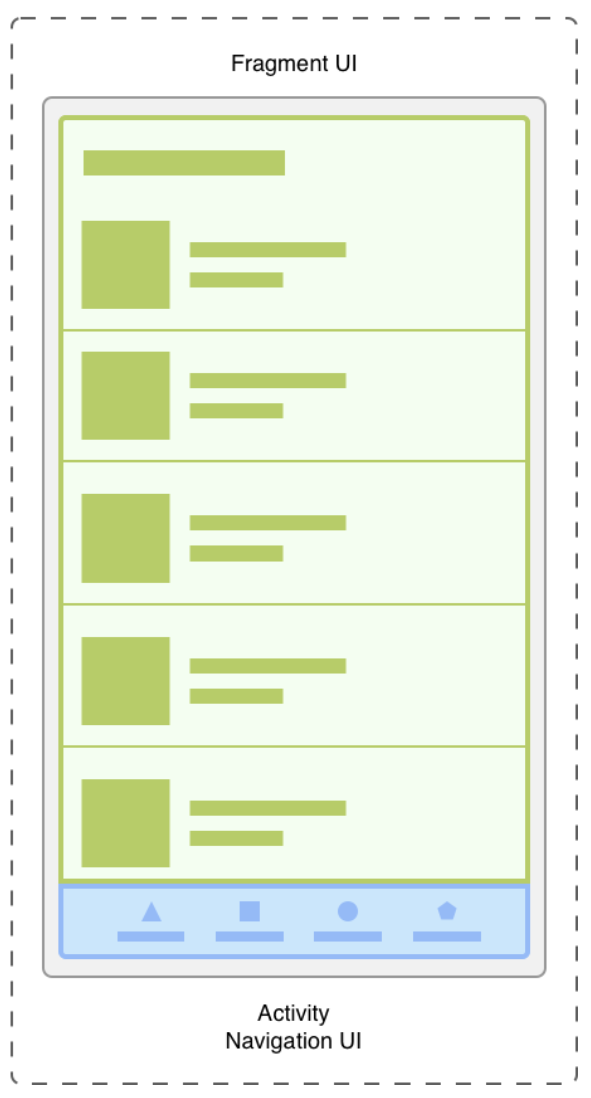
\includegraphics[width=0.4\linewidth]{21-single-activity-architecture.png}
  \caption{Der Aufbau der Applikation im Überblick.}\label{fig:single-activity-architecture}
\end{figure}

\subsection{Navigation}\label{subsec:navigation}

Um die Navigation zwischen verschiedenen Ansichten einer App zu ermöglichen wird von Android die \texttt{Navigation Component}\footnote{Navigation Component. \url{https://developer.android.com/guide/navigation}} der Android-Jetpack Bibliothek bereitgestellt. Diese beinhaltet folgende Teile:

\begin{itemize}
  \item \textbf{Navigationsgraph:} Eine XML-Ressource, die alle Informationen bezüglich der Navigation an einem zentralen Ort enthält. Dazu gehören alle einzelnen Ansichten innerhalb der App, sowie die möglichen Pfade, die ein Benutzer durch Ihre App nehmen kann.
  \item \textbf{NavHost:} Ein leerer Container, welcher die Fragmente der einzelnen Navigationspfade anzeigt. Im Falle der Output App wird die Standardimplementierung \texttt{NavHostFragment} benutzt.
  \item \textbf{NavController:} Ein Objekt, das die App-Navigation innerhalb eines NavHosts verwaltet. Der NavController orchestriert das Austauschen von Zielinhalten im NavHost, wenn Benutzer durch Ihre App navigieren.
\end{itemize}

Sobald der Nutzer innerhalb der App navigiert, wird das entsprechende Fragment der Ansicht im \texttt{NavHost} dargestellt. Dabei stellt die Navigationskomponente auch eine konsistente und vorhersehbare Benutzererfahrung sicher, indem sie sich an einen etablierten Satz von Prinzipien hält. Beispielsweise ermöglicht die Navigation-Komponente die Einbindung der \texttt{BottomNavigationView} mit minimalem Programmieraufwand. Unterstützt wird die Navigation durch \texttt{Safe Args}\footnote{Safe Args. \url{https://developer.android.com/guide/navigation/navigation-pass-data\#Safe-args}}, einem Gradle-Plugin, das Typsicherheit beim Navigieren und Übergeben von Daten zwischen Ansichten bietet. \Cref{fig:navigation} zeigt einen Ausschnitt der grafischen Repräsentation der Navigation innerhalb der App, wobei Pfeile den Navigations-Fluss zwischen Ansichten darstellen.   

\begin{figure}[H]
  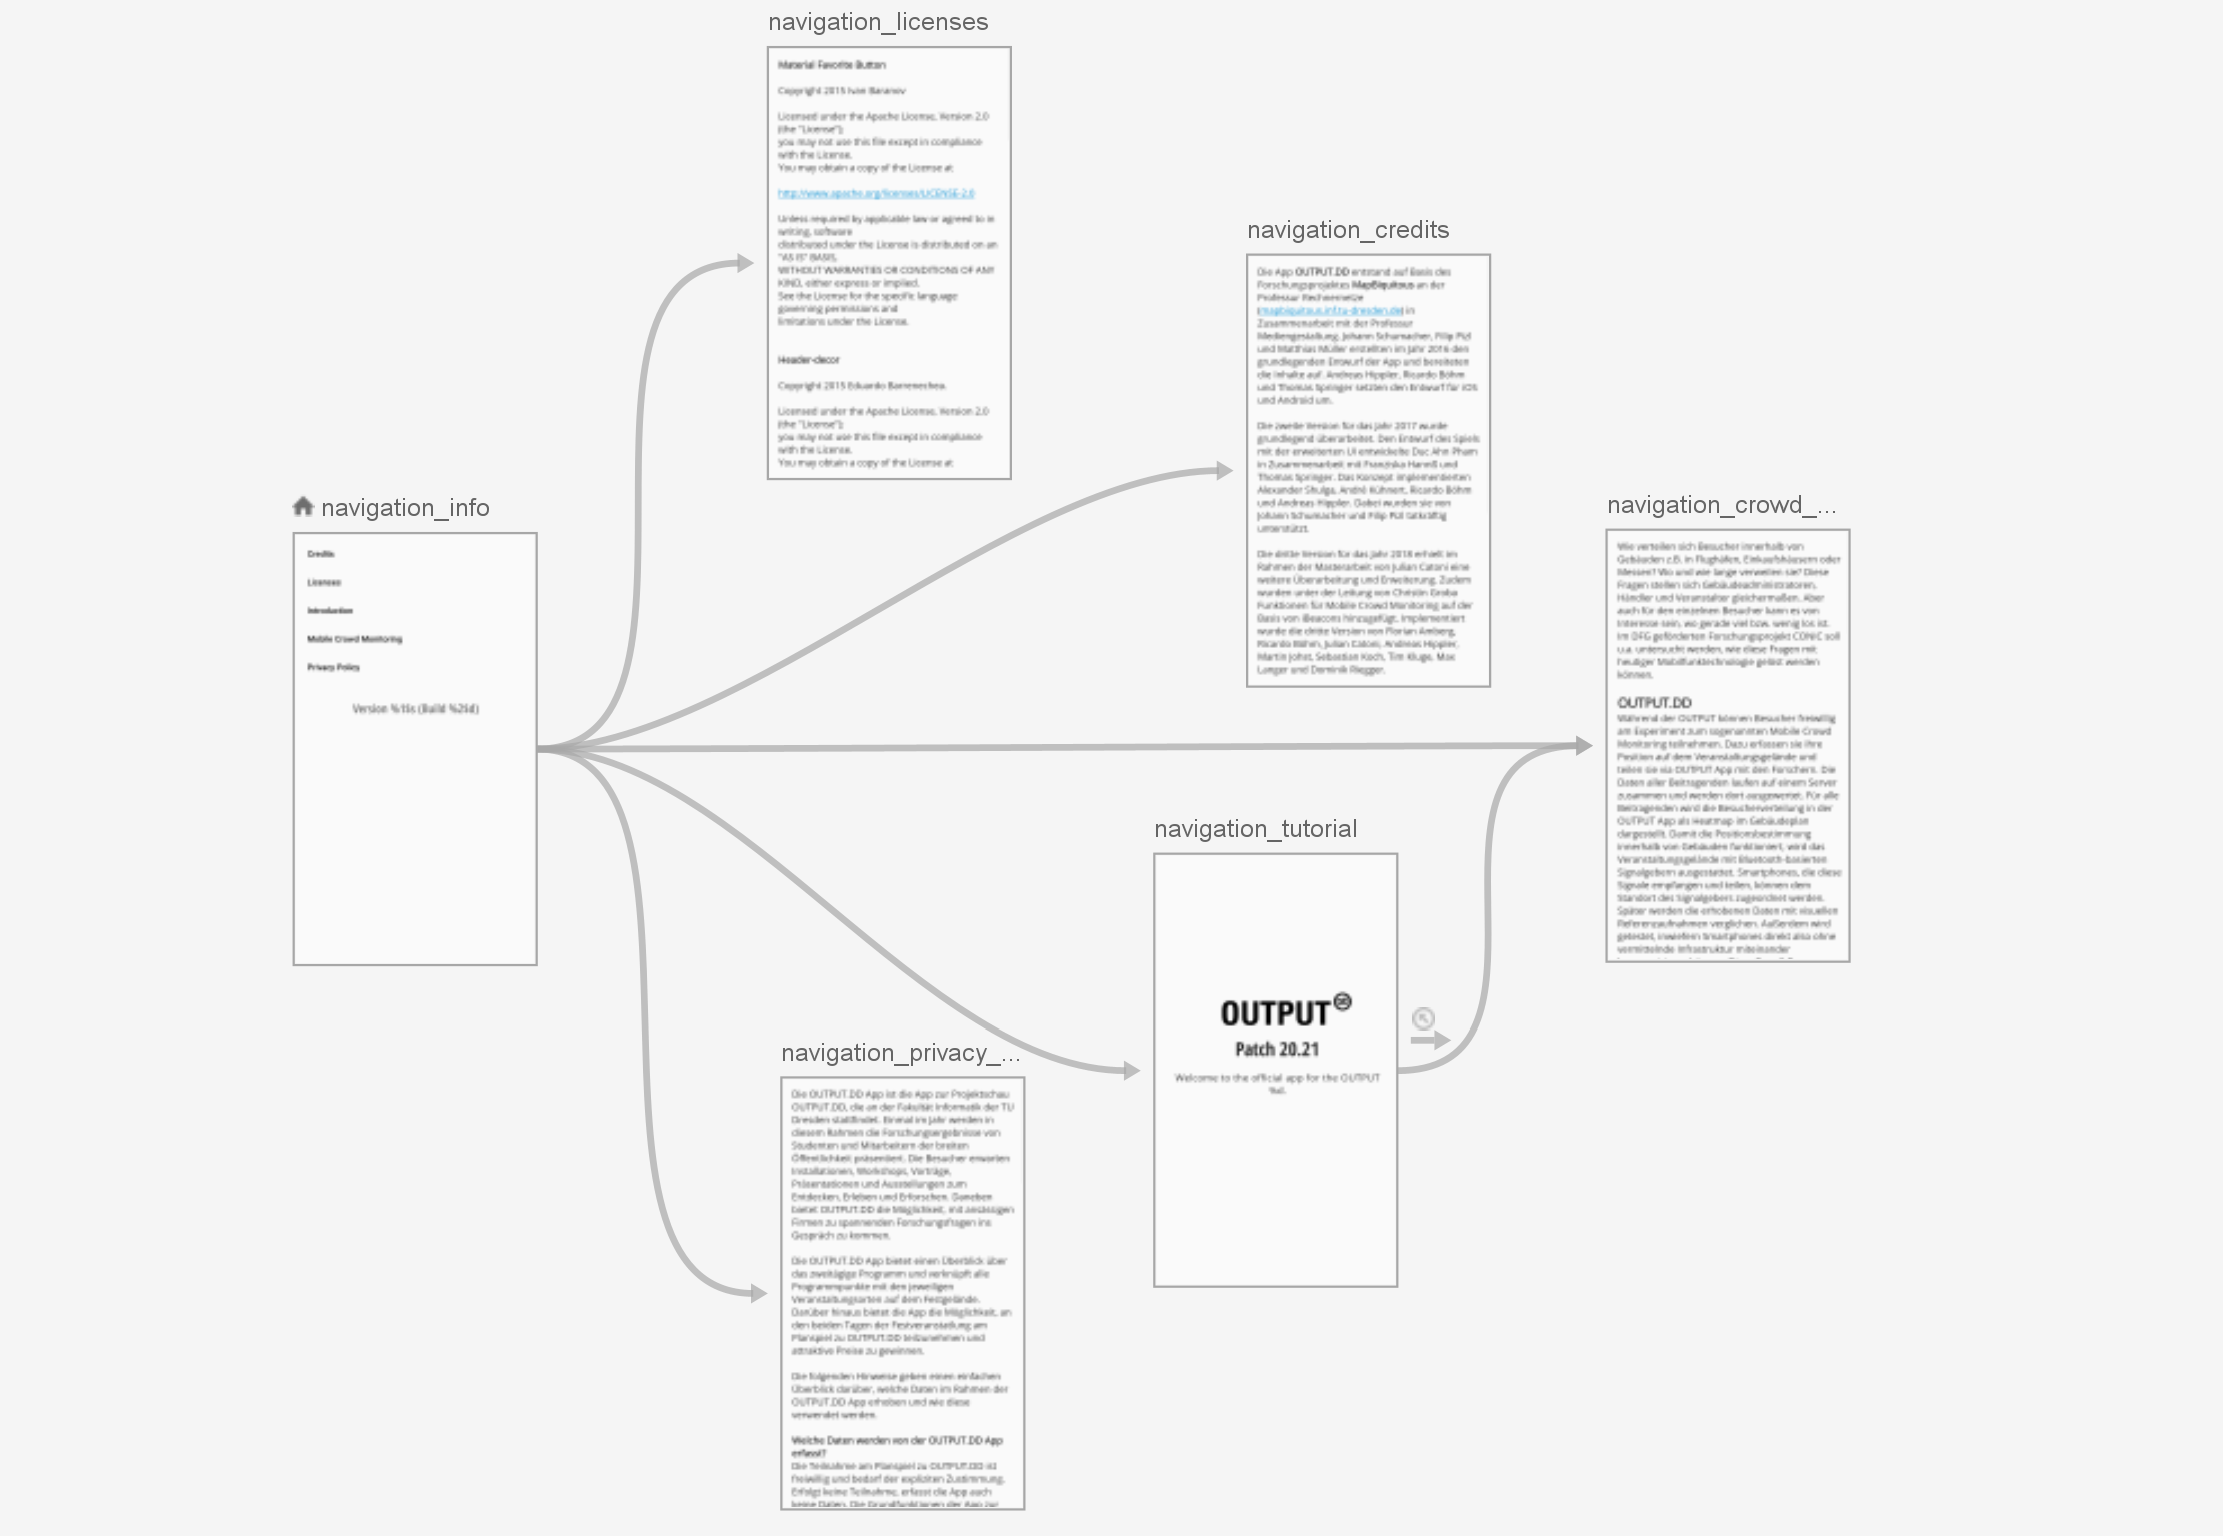
\includegraphics[width=1\linewidth]{22-navigation.png}
  \caption{Ausschnitt der Navigation innerhalb der App.}\label{fig:navigation}
\end{figure}


\subsection{Viewbindung}\label{subsec:viewbinding}

Um einfacher mit den Ansichten interagieren zu können wird eine Technik namens \texttt{Viewbinding}\footnote{Viewbinding. \url{https://developer.android.com/topic/libraries/view-binding}} verwendet. Durch die Aktivierung dieses Build-Features wird automatisch, für jede vorhandene XML-Layout-Datei eine Binding-Klasse erzeugt. Eine Instanz dieser Binding-Klasse enthält direkte Verweise auf alle Ansichten, die eine ID in dem entsprechenden Layout haben. Die Verwendung von Viewbinding erlaubt somit die objektorientierte Verwertung von Views und ersetzt gleichzeitig die Funktionalität der \texttt{findViewById}-Methode. In Bezug auf die in \Cref{lst:layout} gezeigte Layout-Datei ergibt sich die in \Cref{fig:viewbinding} dargestellte Nutzung im Quellcode.

\begin{figure}[H]
    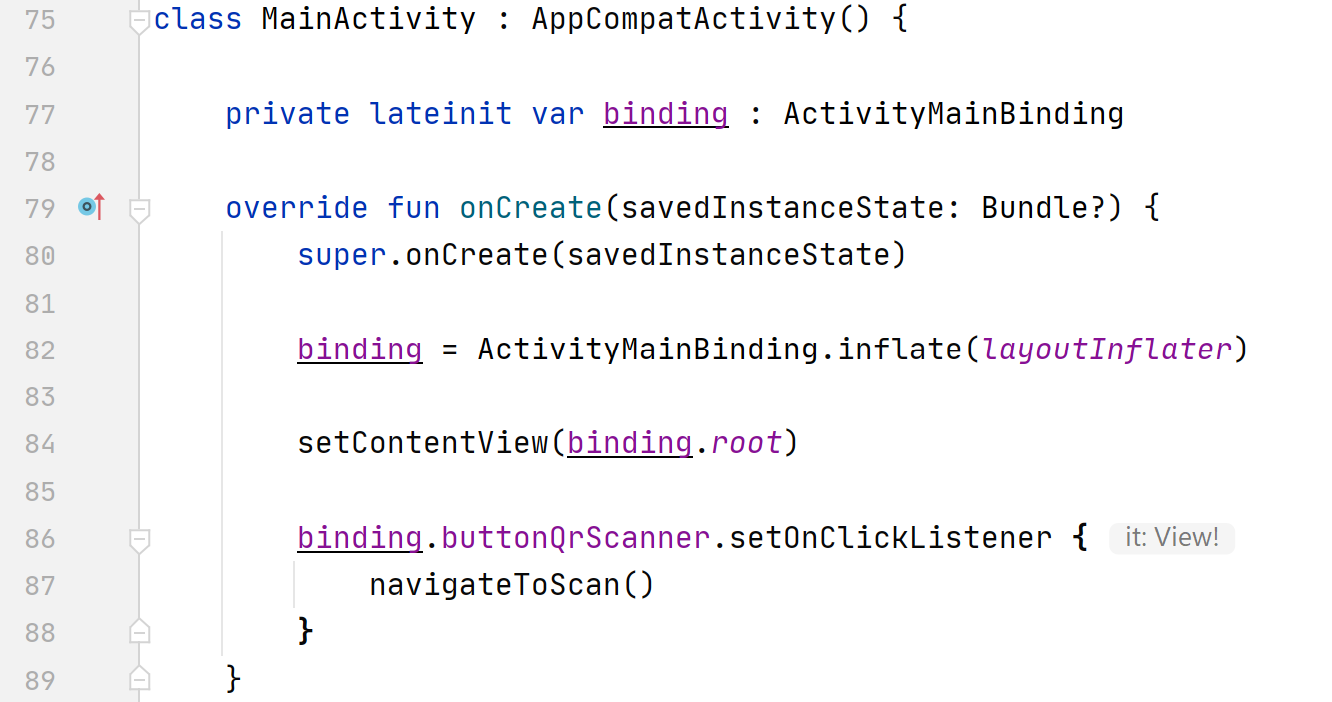
\includegraphics[width=1\linewidth]{23-viewbinding.png}
    \caption{Beispiel für die Nutzung von Viewbinding.}\label{fig:viewbinding}
\end{figure}

\subsection{Databinding}\label{subsec:databinding}

\texttt{Databinding}\footnote{Databinding. \url{https://developer.android.com/topic/libraries/data-binding}} ermöglicht es UI-Komponenten in Layouts an Datenquellen in der App zu binden, indem ein deklaratives Format verwendet wird. Durch die Verknüpfung von Views mit entsprechenden Daten-Variablen können programmatische Aufrufe im Quellcode reduziert werden. Dies führt nicht nur dazu, dass der Code leichter zu pflegen ist, sondern kann auch die Leistung der App verbessern und helfen, Memory-Leaks und Null-Pointer-Exceptions zu vermeiden. Äquivalent zum Fall von Viewbinding werden entsprechende Binding-Klassen automatisch generiert. Im Folgenden werden Variablen innerhalb eines \texttt{data} Blocks im XML-Layout definiert. Diese können anschließend genutzt werden, um die Attribute der Views zu konfigurieren. Die Abbildung der Daten kann sowohl \textbf{unidirektional} als auch \textbf{bidirektional} erfolgen. Die Zuweisung von Variablen erfolgt dabei einmalig zum Zeitpunkt der Initialisierung der View. Sobald sich nun die zugrunde liegenden Daten ändern, wird die View automatisch aktualisiert und erneut gerendert. \Cref{lst:databinding} zeigt die Verwendung von Databinding am Beispiel einer Trophäe in der Spielansicht. Die resultierende Ansicht ist in \Cref{fig:databinding} gezeigt.

\begin{figure}[H]
    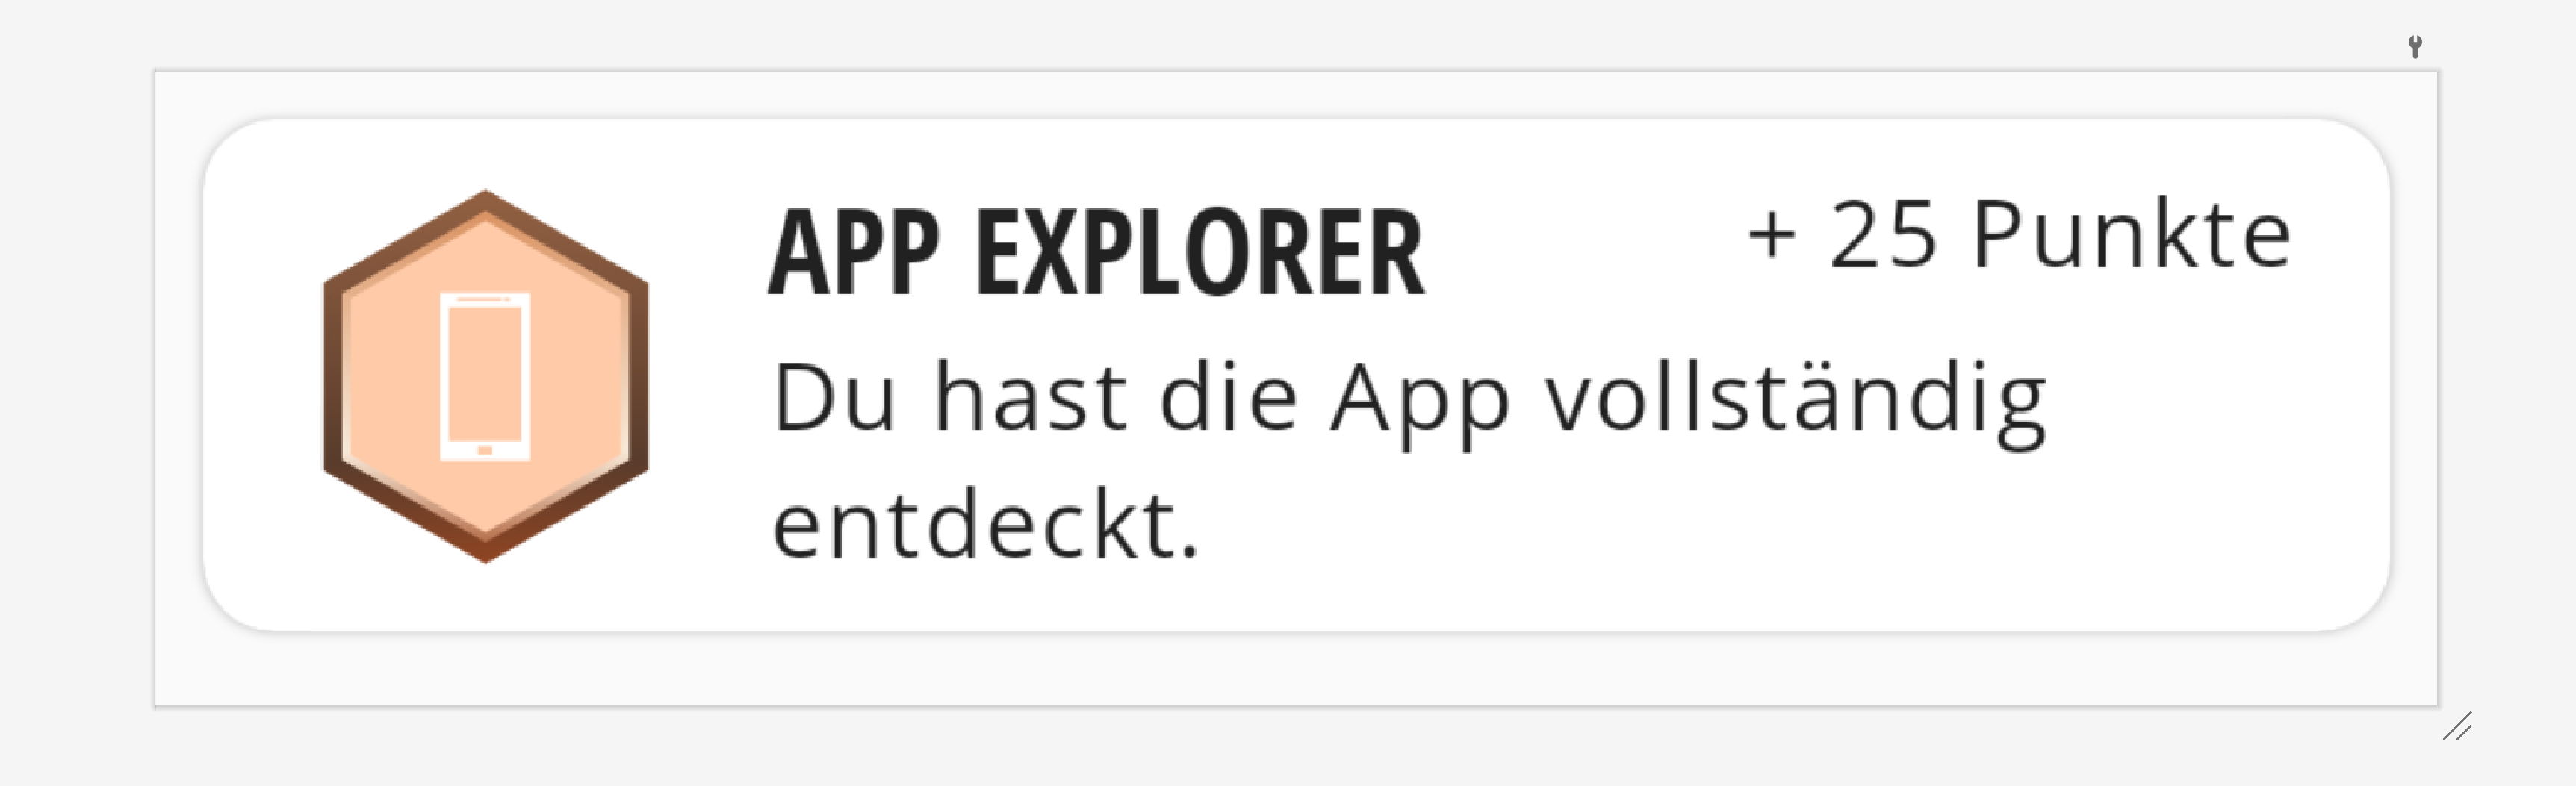
\includegraphics[width=1\linewidth]{24-databinding.png}
    \caption{Darstellung einer Trophäe in der Spielansicht.}\label{fig:databinding}
\end{figure}

\begin{lstlisting}[language=XML, caption={Databinding am Beispiel einer Trophäe in der Spielansicht.}, label={lst:databinding}]
<layout 
    xmlns:android="http://schemas.android.com/apk/res/android"
    xmlns:app="http://schemas.android.com/apk/res-auto">
    <data>
        <variable
            name="achieved"
            type="java.lang.Boolean"/>
        <variable
            name="viewModel"
            type="de.outputdd.database.models.shared.trophy.Trophy" />
    </data>
    <com.google.android.material.card.MaterialCardView ...>
        <androidx.constraintlayout.widget.ConstraintLayout ...>

            <ImageView 
                ... 
                app:bitmap="@{viewModel.icon}"/>

            <TextView
                ...
                android:text="@{viewModel.title}"
                android:enabled="@{achieved}" />

            <TextView
                ...
                android:text="@{String.format("+ %s", viewModel.points)}"
                android:enabled="@{achieved}" />

            <TextView
                ...
                android:text="@{viewModel.details}"
                android:enabled="@{achieved}" />

        </androidx.constraintlayout.widget.ConstraintLayout>
    </com.google.android.material.card.MaterialCardView>
</layout>
\end{lstlisting}

\newpage

\section{Datenfluss- und Architektur-Patterns}

Es werden verschiedene Patterns vorgestellt, die sich im Implementationskonzept wiederfinden und auch Bestandteil der zukünftigen Entwicklung sein sollen. Diese spiegeln ebenso die Prinzipien von Android wider und sind zentraler Bestandteil der App.

\subsection{View-Model-ViewModel-Pattern}

\textbf{Model-View-ViewModel (MVVM)} ist eine Variante des bekannten Model-View-Presenter (MVP) Entwurfsmusters. Das Ziel dieses Architektur-Patterns ist die Trennung von Darstellung und Logik der Benutzeroberfläche. Die Bestandteile des Patterns sind:

\begin{itemize}
    \item \textbf{Model:} Eine Instanz welche die Daten der Anwendungsdomäne enthält. Diese Objekte haben keinen direkten Zusammenhang zur View, sondern repräsentieren Datenbank-Objekte im Kontext der Anwendung.
    \item \textbf{View:} Die Repräsentation einer Ansicht, ohne jegliche Anwendungslogik.
    \item \textbf{Viewmodel:} Die Schnittstelle zwischen den Daten im Anwendungskontext und der Repräsentation. Viewmodels stellen die Daten der Models als Datenfluss für die View bereit. 
\end{itemize}

\Cref{fig:mvvm} zeigt den Aufbau des MVVM-Patterns. Bekannte CRUD-Operationen auf den Daten werden dabei durch das Viewmodel ausgeführt. In den meisten Fällen verfügt das Model über Mechanismen um gezielt auf Änderungen der Daten reagieren zu können. Die Daten können anschließend vom ViewModel als Datenfluss für die View bereitgestellt werden. View und ViewModel verfügen über eine unidirektionale oder bidirektionale Bindung, bei welcher die View die Daten sowie Methoden des Viewmodels referenziert. Gleichzeitig kann ein gegebenes ViewModel für mehrere Views eingesetzt werden.

\begin{figure}[H]
    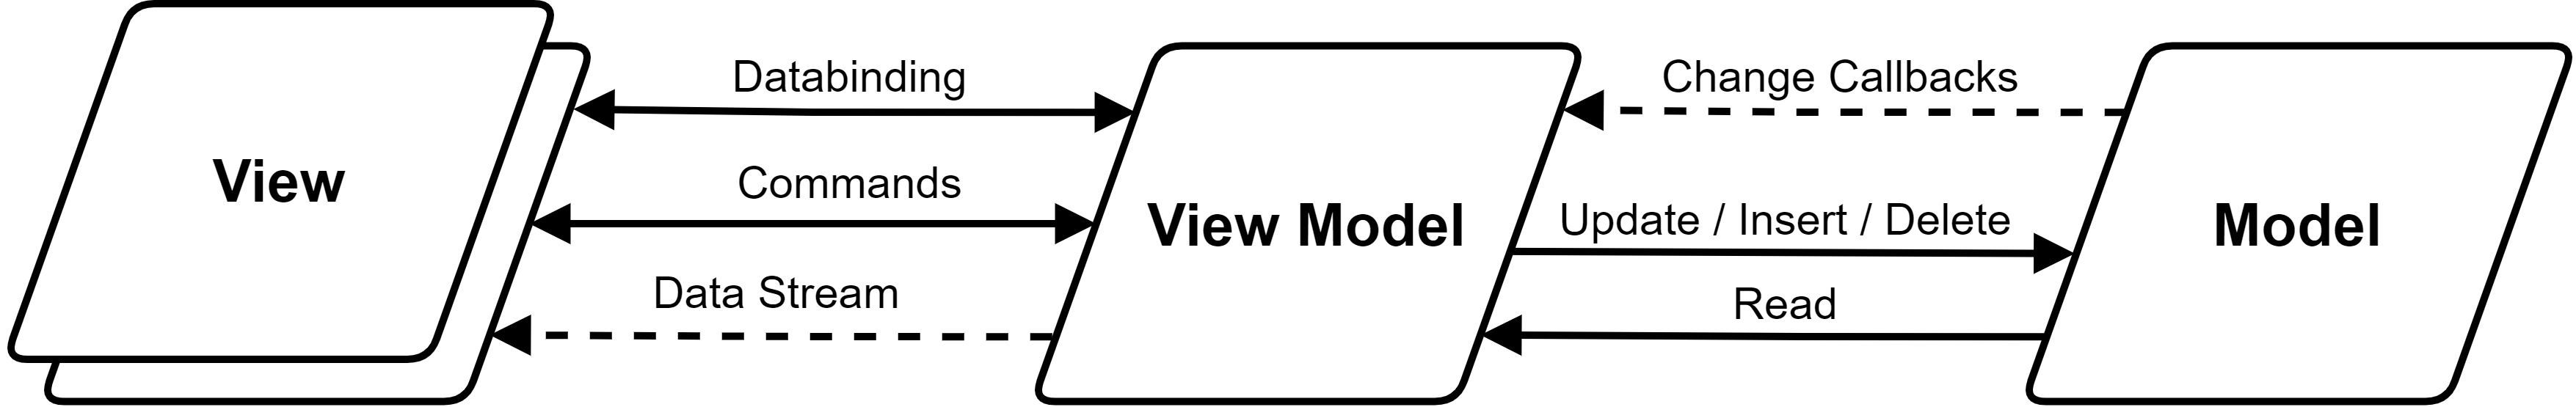
\includegraphics[width=1\linewidth]{25-model-view-viewmodel.png}
    \caption{Aufbau des Model-View-ViewModel-Pattern.}\label{fig:mvvm}
\end{figure}

\newpage

\subsection{Observer-Pattern}\label{sub:observer}

Das \textbf{Observer-Pattern} ist ein weiteres Entwurfsmuster, welches in der Android-Entwicklung eine zentrale Rolle spielt. Es gehört zur Kategorie der Verhaltensmuster und dient zur Weitergabe von Änderungen an abhängige Datenstrukturen. Damit lassen sich Ereignis-basierte Abläufe programmieren. In der für die Android-Entwicklung üblichen Variante des Observer-Patterns, informiert ein Objekt (genannt \texttt{Subjekt}) alle  abhängigen Objekte (genannt \texttt{Observer}) von Änderungen und überträgt dabei jeweils eine aktuelle Kopie der Daten als Parameter. Der Ablauf ist in \Cref{fig:observer} gezeigt. Diese Form wird auch \enquote{Push-Update Observer} genannt. 

\begin{figure}[H]
    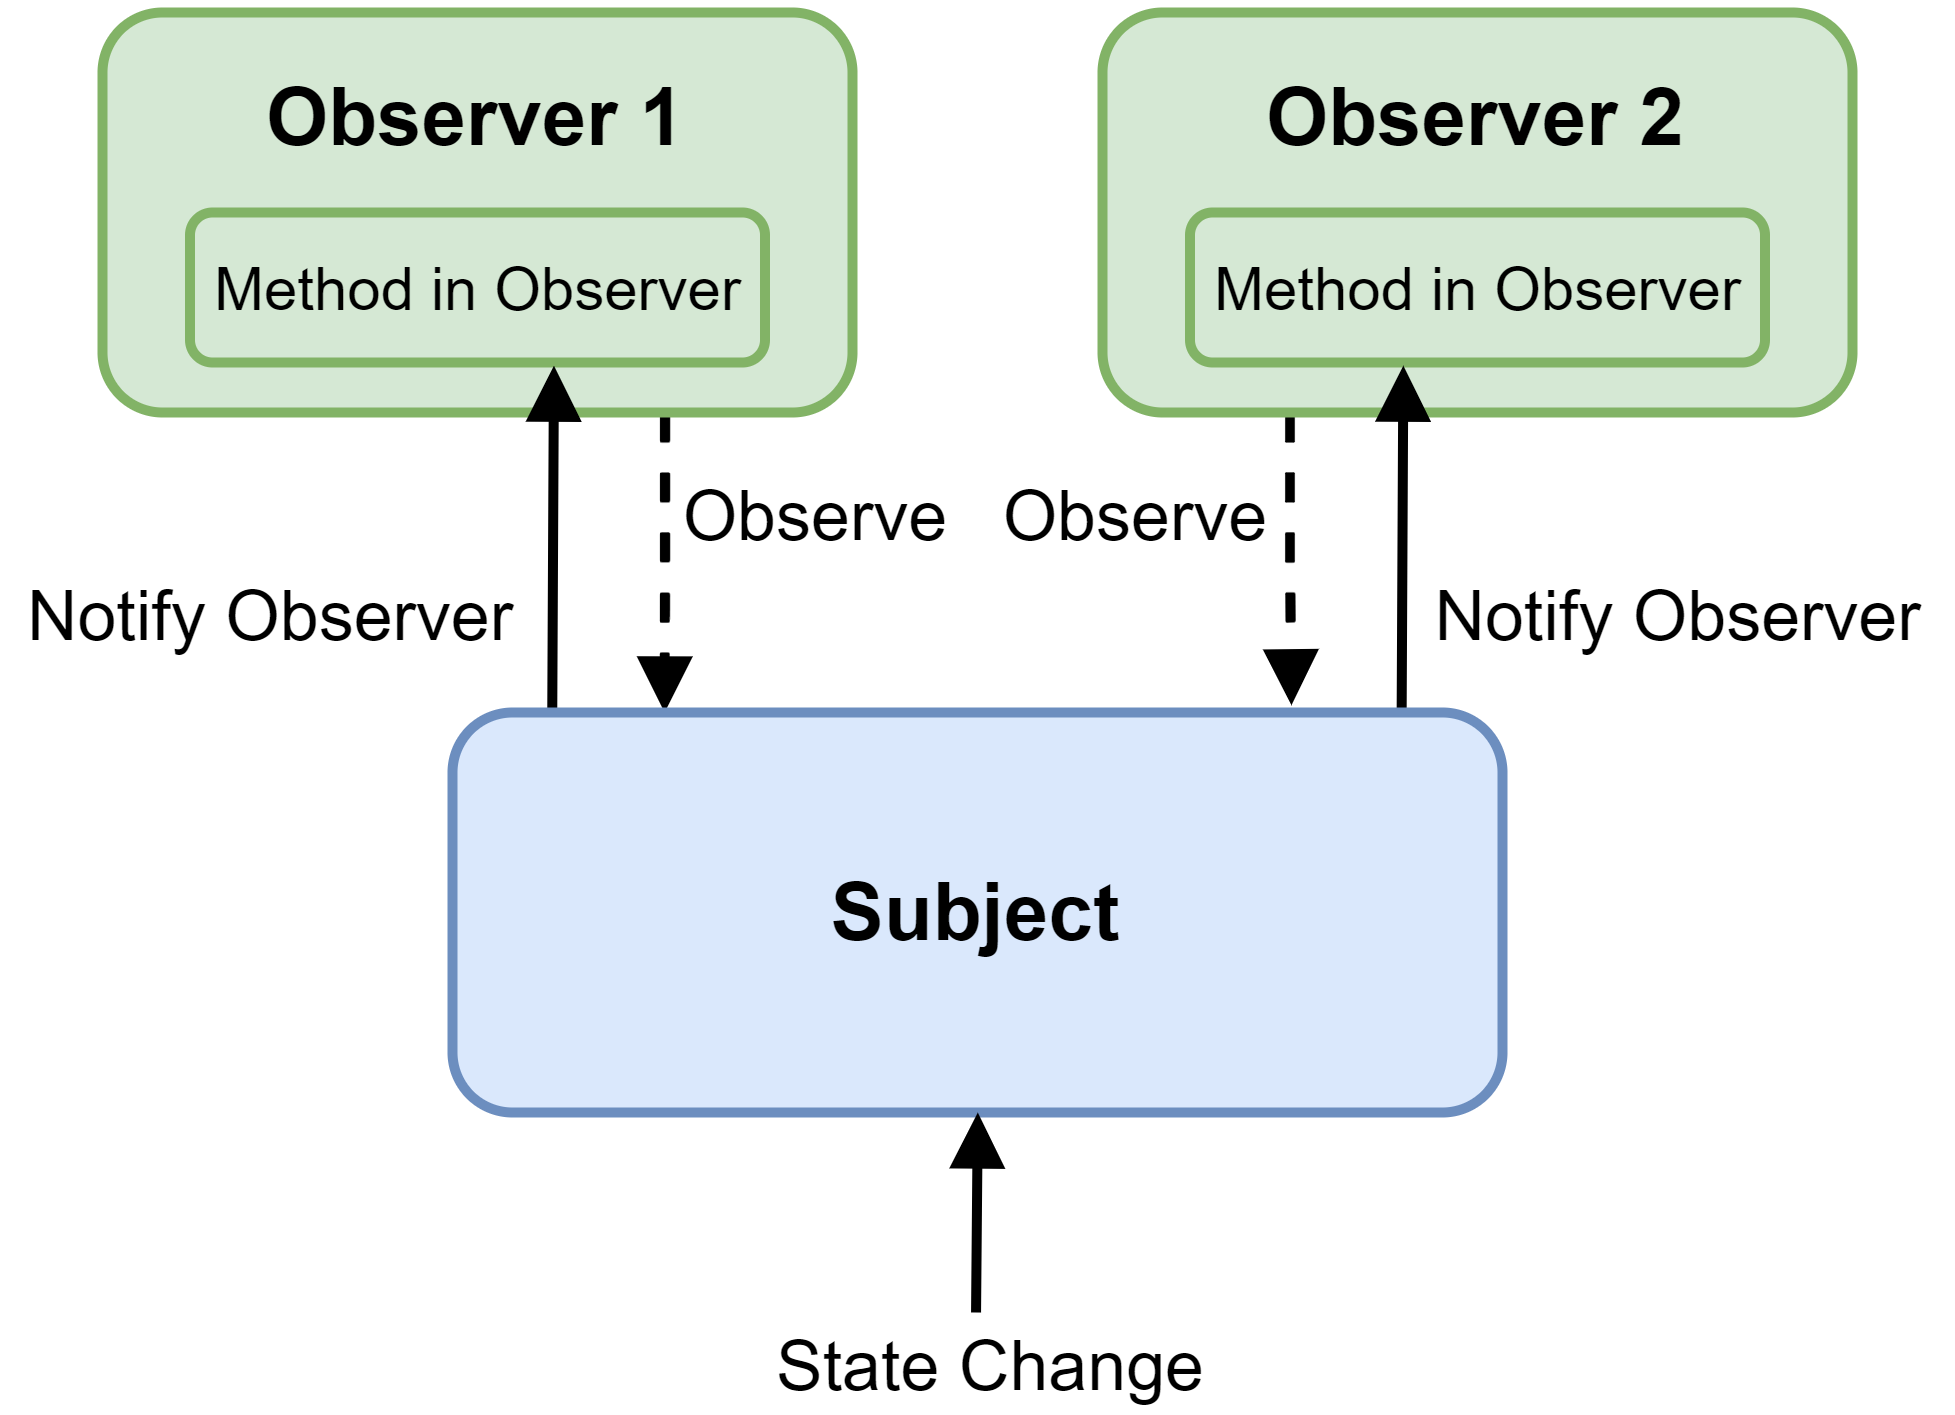
\includegraphics[width=0.55\linewidth]{26-observer.png}
    \caption{Aufbau des Observer-Pattern.}\label{fig:observer}
\end{figure}

\subsection{Delegation-Pattern}\label{subsec:delegation}

Das \textbf{Delegation-Pattern} ist ein strukturelles Entwurfsmuster, welches die Bildung von Objekten erleichtert und damit als Alternative zur Vererbung die Wiederverwendung von Implementationen erlaubt. Das Prinzip des Patterns beruht auf der Weitergabe von Aufrufen (Delegation) an ein weiteres Objekt. Die Auswertung des Zugriffs geschieht im Falle von \texttt{Delegation} im Kontext des initialen Objektes. Damit grenzt sich das Prinzip von \texttt{Delegation} klar gegenüber dem Prinzip von \texttt{Forwarding} ab, wobei die Auswertung des Zugriffes im Kontext des Objektes geschieht, an welches delegiert wurde. Das Pattern wird nativ von der Programmiersprache \hyperref[sec:kotlin]{Kotlin} unterstützt und kann somit ohne weiteres direkt als Element der Programmiersprache verwendet werden. Kotlin unterstützt dabei sowohl die Delegation von Interfaces\footnote{Delegation. \url{https://kotlinlang.org/docs/delegation}} sowie die Delegation von einzelnen Eigenschaften\footnote{Delegated Properties. \url{https://kotlinlang.org/docs/delegated-properties.html}}.

\begin{figure}[H]
    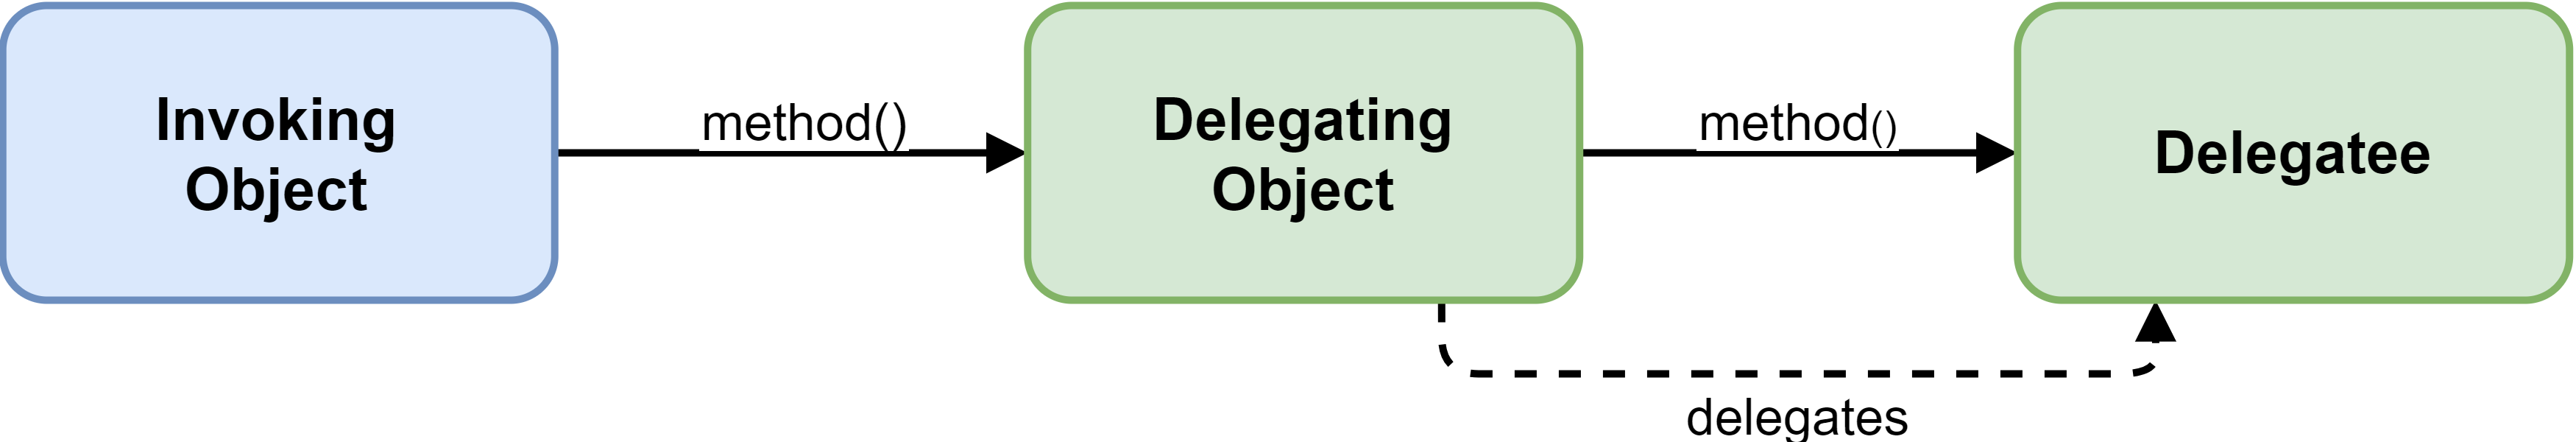
\includegraphics[width=1\linewidth]{27-delegate.png}
    \caption{Aufbau des Delegation-Pattern.}\label{fig:delegation}
\end{figure}


\subsection{Mediator-Pattern}

Wie auch das \hyperref[sub:observer]{Observer-Pattern} zählt das \textbf{Mediator-Pattern} zu der Klasse von Verhaltensmustern. Das Mediator-Pattern richtet sich dabei an den Informationsaustausch zwischen Objekten. Die Kommunikation findet mittels eines sogenannten \texttt{Mediator}-Objekts statt, welches als Schnittstelle zwischen den beteiligten Objekten dient. Dadurch kann das kooperative Verhalten zentral verwaltet werden, wobei die Implementierung des \texttt{Mediator} unabhängig von der Implementierung der beteiligten Objekte erfolgen kann. Somit kann eine lose Kopplung geschaffen werden, was zugleich die Komplexität der Kooperation mindert. 

\begin{figure}[H]
    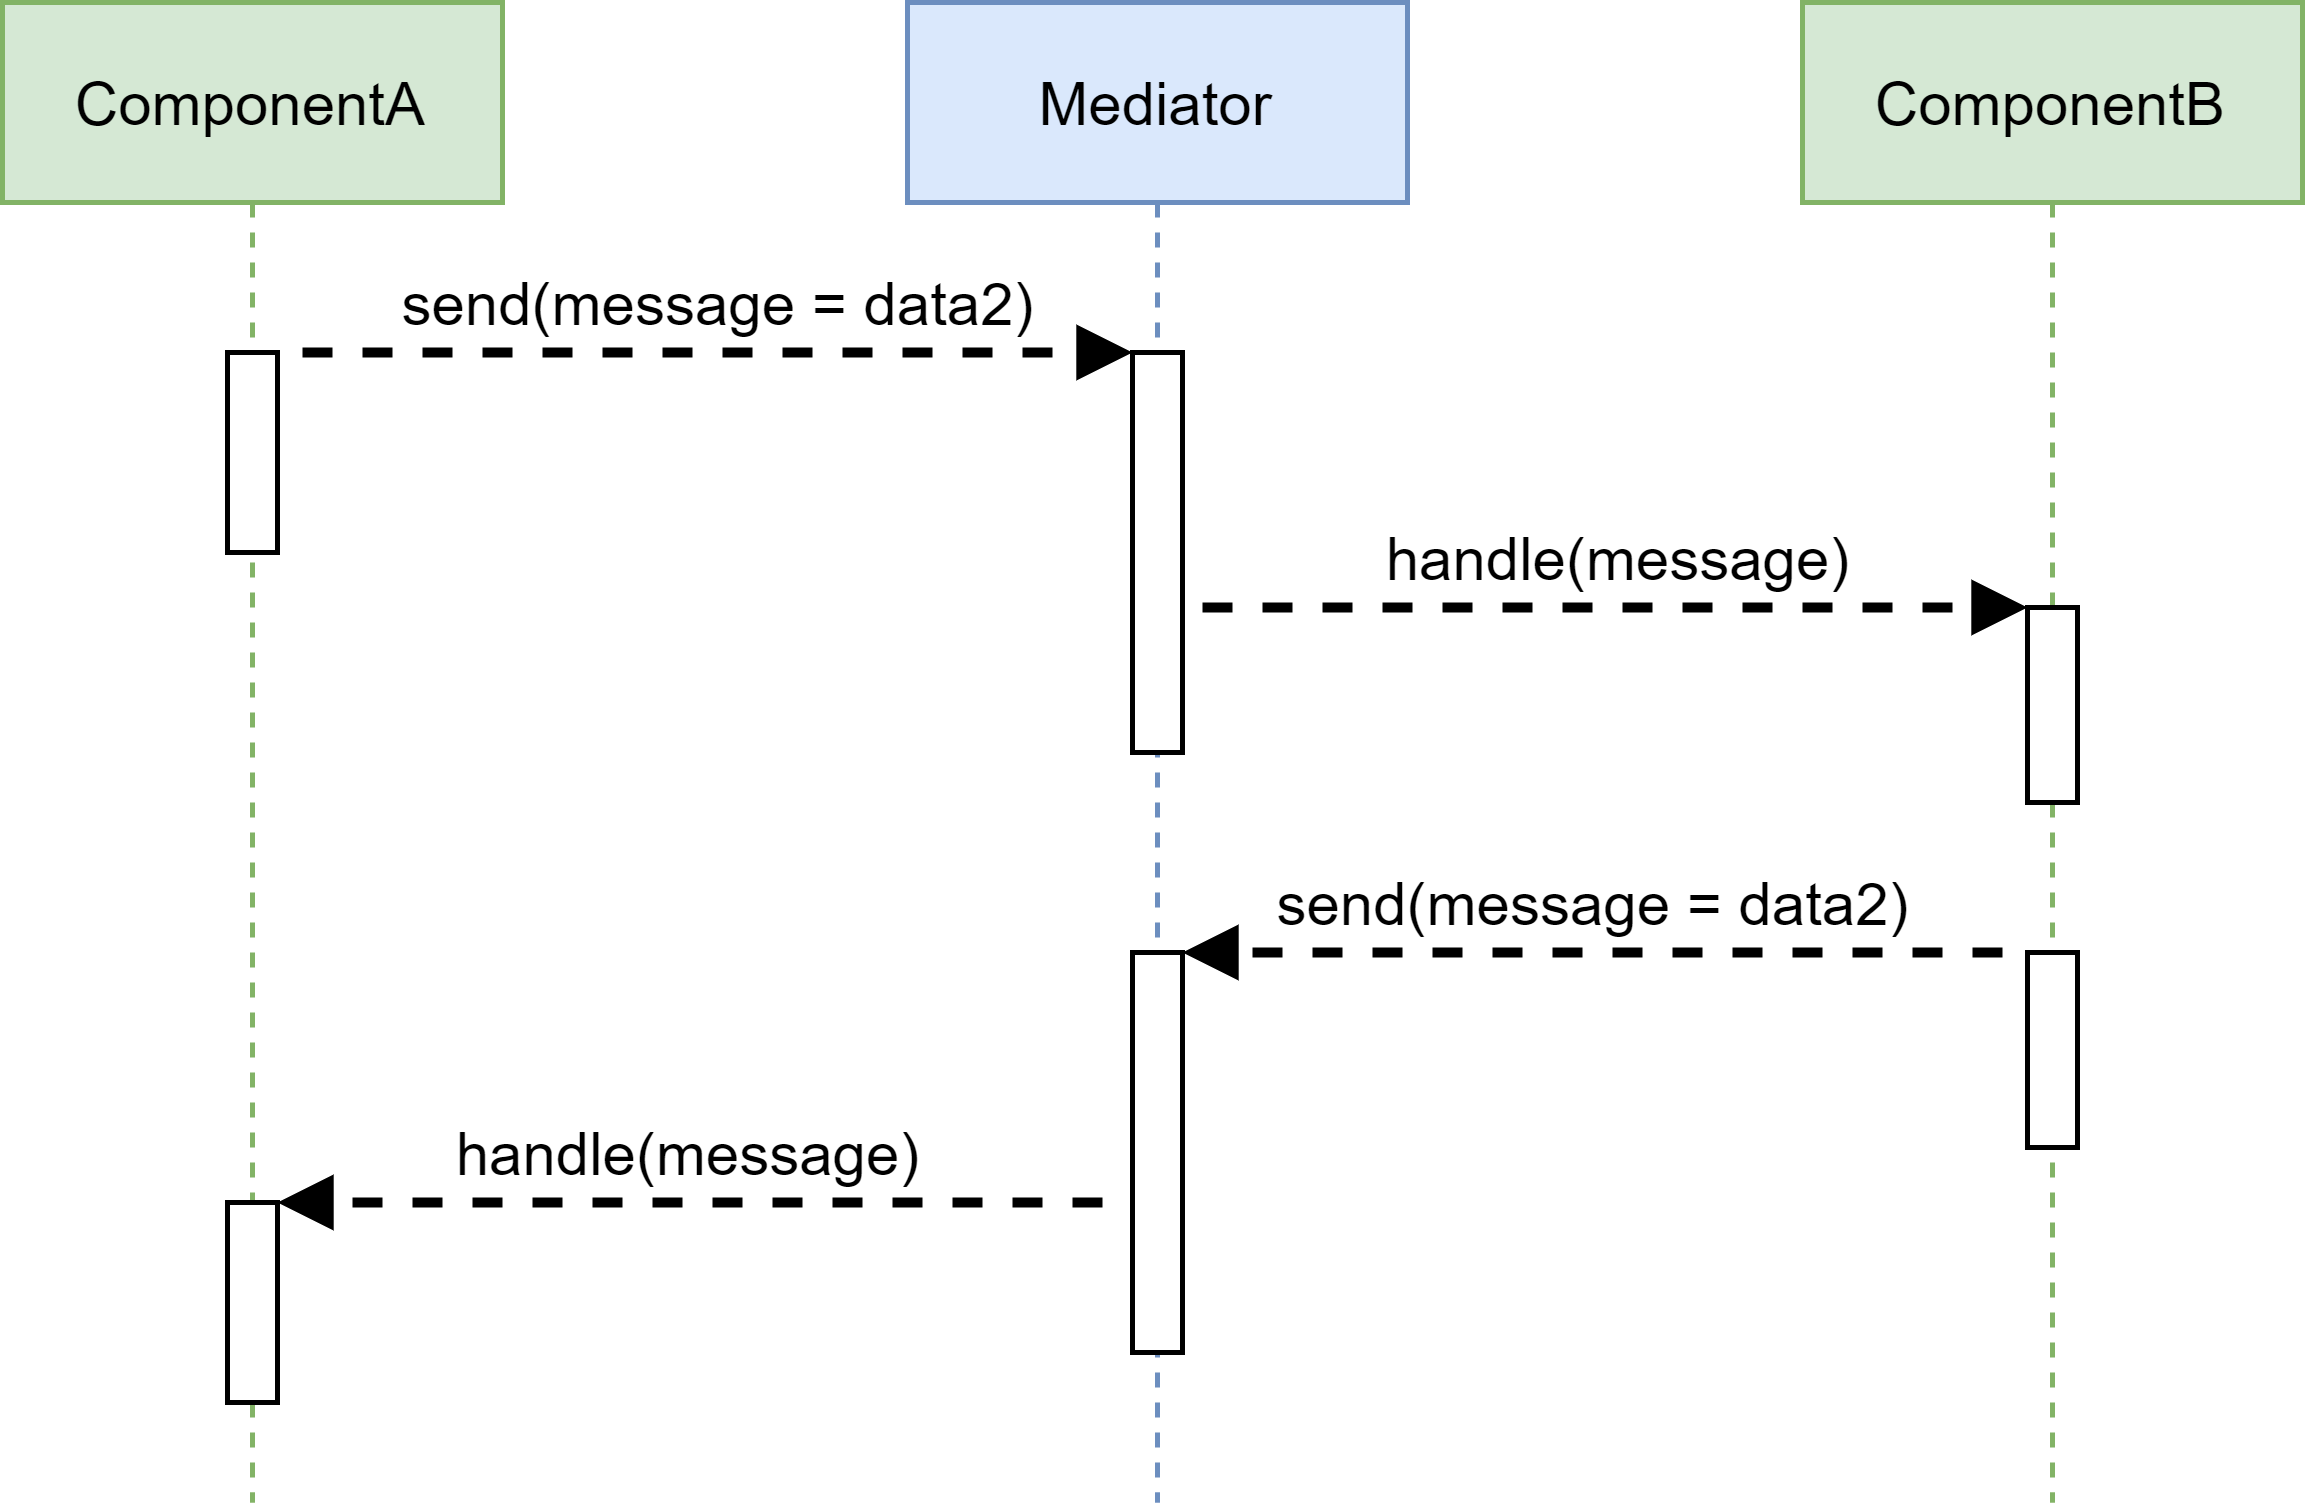
\includegraphics[width=0.85\linewidth]{28-mediator.png}
    \caption{Ablaufdiagramm des Mediator-Pattern.}\label{fig:mediator}
\end{figure}

  \chapter{Analyse}\label{ch:analyse}
  \chapter{Konzept und Implementation}\label{ch:konzept}

  \chapter{Zusammenfassung}\label{ch:zusammenfassung}

Im Verlauf des Sommersemester 2020 wurde ein Framework für das Couchbase-Framework erstellt, welches das bestehende Realm-Framework in der OUTPUT.DD App ersetzen sollte. Während einer Analyse der Apps konnten zahlreiche strukturelle Probleme und Antipatterns in der bestehenden identifiziert. Aus diesem Grund war es Aufgabe dieser Projektarbeit, eine umfängliche Neuimplementation der App inklusive der Integration des Datenbank-Frameworks durchzuführen. Hierbei sollten die in \Cref{ch:einleitung} beschriebenen Probleme beseitigt werden. Gleichzeitig wurden verschiedene Strategien entwickelt die das Wiedereintreten dieser Probleme verhindert. 

\paragraph{Vorgehensweise und Ergebnisse} Hierfür wurden in \Cref{ch:grundlagen} verschiedene Entwurfsmuster beschrieben sowie deren Anwendungsbereiche diskutiert. Durch die Nutzung dieser Design-Patterns wurden signifikante Vorteile für die Separabilität, Funktionalität und Erweiterbarkeit erreicht. Gleichzeitig konnte die Struktur der App analysiert und eine Top-Level-Architektur geschaffen werden, welche die Zerlegung in Teilbereiche der App erlaubt. Durch die Verwendung von statischen Analysetools konnte Codequalität gesteigert und das Eintreten von \enquote{Code Smells} unterbunden werden. Die Neuimplementation der App orientiert sich an bekannten Prinzipien der Usability. Genauso wurde auf die Einhaltung der OUTPUT.DD Corporate Identity geachtet. Gleichzeitig wurde eine Modernisierung der Ansichten durchgeführt und unter Absprache im Projektteam ein optionales dunkles Design eingeführt. Um redundanten Arbeitsaufwand zu minieren wurde auf eine modulare Entwicklung von UI-Komponenten gesetzt, wodurch die Wiederverwendbarkeit von Elementen gewährleistet wurde. Damit konnte die Geschäftslogik der einzelnen Ansichten weiter voneinander separiert werden. Für die Gamification wurden Modelle und Basisalgorithmen entwickelt, um die Errungenschaften weitestgehend unabhängig von den beteiligten UI-Komponenten implementieren zu können. Zum Testen der App wurden konkrete Strategien entwickelt und ein Docker-basiertes Deployment geschaffen. Für die Weiterentwicklung des Projektes wurden neben dieser Dokumentation auch weitere Leitfäden in den Git-Repository der Apps erstellt.

\newpage

\paragraph{Offene Punkte} Die Neuimplementation der OUTPUT.DD-Apps konnte vollständig durchgeführt werden. Neben der Beseitigung von zahlreichen Problemen konnte eine technische und optische Modernisierung der Funktionalitäten umgesetzt werden. Lediglich bei der Integration des Crowd-Monitoring-Framework wurden zahlreiche Probleme identifiziert, die nicht im Rahmen dieser Projektarbeit behoben werden konnten und stattdessen im Fokus zukünftiger Projektarbeiten stehen werden. Im Hinblick auf die OUTPUT.DD 2021 am 8. Juli 2021 werden die Apps weiterhin getestet und Verbesserungen und Optimierungen umgesetzt. Auch die Distribution der Apps und das Deployment auf einem Produktionssystem für OUTPUT.DD 2021 wird noch im Rahmen des Supportprozesses zukünftiger Teil dieser Arbeit sein.

\paragraph{Danksagung}
Diese Projektarbeit hat mir persönlich sehr viel Spaß bereitet. Gleichzeitig konnte ich weitere Kenntnisse im Bereich App-Development sammeln. Besonderen Dank möchte ich Dr. Thomas Springer für die Betreuung dieser Projektarbeit und die zahlreichen Hinweise aussprechen. Außerdem möchte ich meinem guten Freund Philipp Matthes für den sehr konstruktiven Entwicklungsprozess, die Umsetzung der iOS-App und die sehr interessanten Gespräche danken.


  \newpage

  % use lowercased roman page numbers for the appendix and the bibliography
  \pagenumbering{roman}

\end{document}
